\documentclass[11pt,titlepage]{article}

\usepackage{geometry}
\usepackage{float}
\usepackage{graphicx}
\geometry{a4paper}
\geometry{margin=2cm}
\geometry{portrait}

\newcommand{\horrule}[1]{\rule{\linewidth}{#1}}

\title{
		\normalfont \normalsize \textsc{COS 330} \\
		%\normalfont \normalsize \textsc{Project Name: KinderFinder} \\ [25pt]
		\horrule{0.5pt} \\[0.4cm]
		\huge Practical 4\\
		\horrule{2pt} \\[0.5cm]
}
\author{\begin{tabular}{rl}
	\texttt{Student Name:} & \texttt{} \\[0.5cm]
	Uteshlen Nadesan & 28163304 \\
\end{tabular}
	\\ \\ \texttt{Version: 0.1}
%	\\ \\ \texttt{Change History:}
%	\\ The Summary here.
	}
\date{30/09/2014} 

\begin{document}
\maketitle
\tableofcontents
\newpage

\section{Task 1}

\subsection{Hashcat command line with parameters used. [4]}
%\begin{figure}[H]
%\begin{center}
%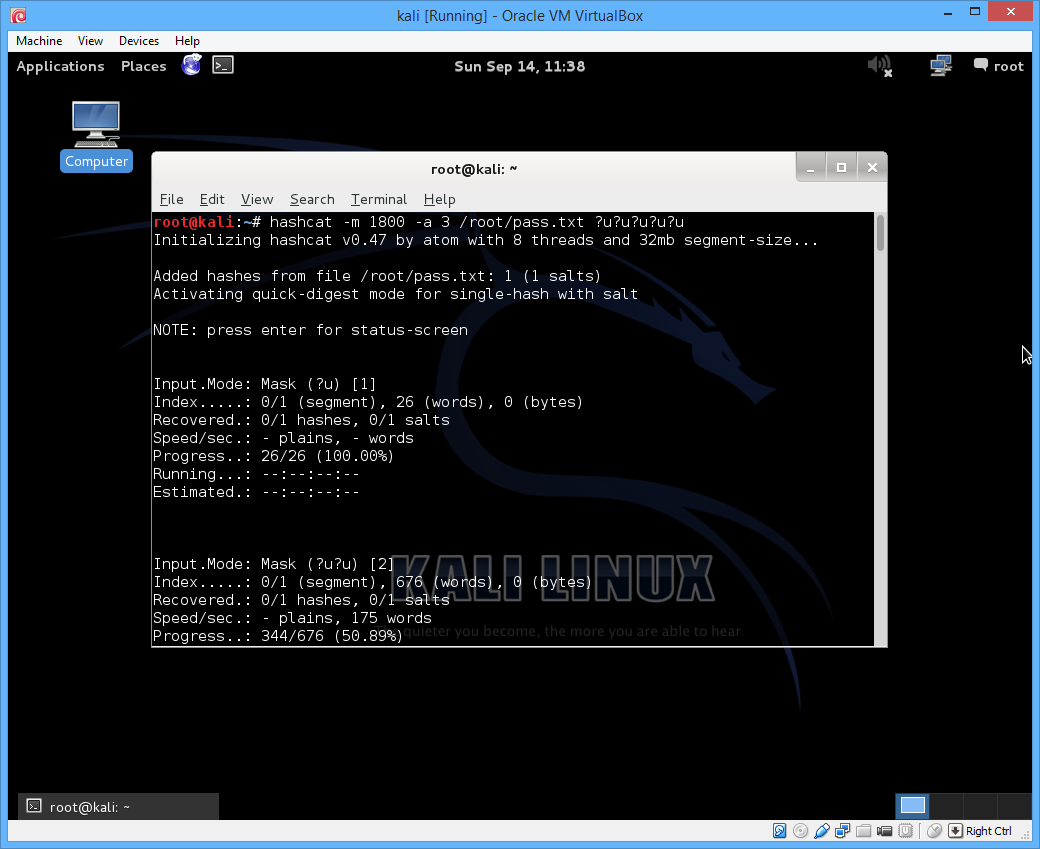
\includegraphics[scale=0.6]{task1b.png}
%\caption{task 1b}
%\end{center}
%\end{figure}

\end{document}

